\section{Introduction}\label{sec:intro}
zbMATH classified more than 135k articles in 2019 according to the Mathematics Subject Classification~(MSC)~\cite{Khnemund2016}.
With more than
\href{https://zbmath.org/classification/}%
{6600} class labels, this classification task requires significant depth-knowledge of the particular fields of mathematics in order to obtain correct fine-grained MSC codes of the articles.
Therefore the classification procedure is two-fold.
At first, the articles are pre-classified into one of \href{https://msc2020.org}%
{63} coarse-grained MSC subject numbers, which are the two first digits of the first MSC code of each article.
In a second step, subject editors assign fine-grained MSC codes in their area of expertise.

In this paper, we focus on the coarse-grained classification of the \emph{primary MSC subject number} (pMSCn) and explore how modern machine learning technology can be employed to automate this process.
In particular, we compare the current state of the art technology with a system customized for the application in zbMATH from 2014~\cite{SchonebergS14}.
We formulate the following research questions:
\begin{enumerate}
  \item Which measures are best to assess the quality of classifications?
  \item Do mathematical formulae improve the quality of the classifications?
  \item Does the Part of Speech preprocessing improve the quality of classifications?
  \item Which features are most important for the correct classification?
  \item How does the currently best method perform?
  \item How does this compare to a human baseline?
\end{enumerate}
\section{Method}\label{sec:method}
\smartdiagramset{back arrow disabled=true}
  \smartdiagram[flow diagram:horizontal]{Generate zbMATH dataset, match with MR data, train methods, test methods, evaluate results}


To investigate the given problem, we first create a test and training dataset.
Second we investigate different encodings, train our models and evaluate the results.
\subsection{Generation of a test and training dataset}
\paragraph{Filter current high quality articles:}
The zbMATH database has assiged MSC codes to more than
\href{https://zbmath.org/?q=cc%3A*}%
{3.6 M} articles.
However, the way how mathematical articles are written changed in the last century and the classification of historic articles is not something we aim to investigate in this article.
The first MSC was created in 1990 and updated every ten years (2000, 2010, and 2020)~\cite{MSC2010}.
With each update automated rewrite rules are applied to map codes from the old MSC to the next MSC version, with is connected with a loss of accurancy of the class labels.
To obain a coherent and high qualtiy dataset for training and testing, we focused on recent articles from the years 2000 to 2019 classified using the MCS verion 2010 and considered only selected journals.
Moreover, we restricted the article selection to articles in English and limited ourselves to abstracts rather than reviews of articles.
To be able to compare methods that are based on references and methods that use text and title, we only selected articles that have one reference that
can be matched to another article.
In addition, we excluded articles that are not finally published and processed. The list of articles is availible from our website: \url{https://automsceval.formulasearchengine.com}
\paragraph{Splitting to test and training set:}
After applying all these filters, we split the resulting list of 442'382 articles into a test and training set.
For the test set we strive to measure the bias of our zbMATH classification labels.
Therefore, we used the articles of, which we knew the classification labels by the MR service as training set.
The resulting test set consists of $n=32'230$ articles and the training set of 410'152 articles.
To ensure that this selection does not introduce additional bias, we did also compute standard ten-fold cross validation, cf. Section 3.
\paragraph{Definition of article data format}
To maximize reproducibility, we created a dedicated dataset from our article selection, which we aim to share with other researchers.
However, currently, legal restrictions apply and the dataset can not yet be provided for anonymous download at this date.
Each of the 442'382 articles in the dataset has the following fields:
\begin{description}
  \item[de] An eight digit ID of the document\footnotemark.
  \item[labels] Actual MSC codes\footnotemark[\value{footnote}].
  \item[title] The English title of the document, with LaTeX macros for math~\cite{Schubotz2019b}.
  \item[text] The text of the abstract with LaTeX macros.
  \item[mscs] A comma seperated list of MSC codes generated from the references.
\end{description}
\footnotetext{The field \texttt{de} and \texttt{labels} must not be used as input to the classification algorithm.}
These 6 fields were provided as CSV files to the algorithms.
Here, the \texttt{mscs} field was generated as follows: For each reference in the document we look up the MSC codes of the reference. For example, if document has 3 references $A,B,C$ that are also in the also documents in zbMATH and the MSC codes of $A,B,C$ are $a_1$ and $a_2$, $b_1$, and $c_1-c_3$ the field mscs reads $a_1  a_2, b_1, c_1 c_2 c_3.$


After training we require each algorithm to return the following fields in CSV format for the testset:
\begin{description}
  \item[de (integer)] Eight digit ID of the document.
  \item[method (char(5))] Five letter ID of the run.
  \item[pos (integer)] Position in the result list.
  \item[coarse (integer)] Coarse-grained MSC subject number.
  \item[fine (char(5), optional)] Fine-grained MSC code.
  \item[score (numeric, optional)] Self-confidence of the algorithm about the result. 
\end{description}
We enforce that the fields \texttt{de}, \texttt{method} and \texttt{pos} form a primary key, i.e., there can not be two entries in the result with the same combination of values.
Note that for the current multiclass classification problem \texttt{pos} is always 1 as only the primary MSC subject number is considered.
\subsection{Definition of evaluation metrics}
While the assignment of all MSC codes to each article is a multi-label classification task, the assignment of the primary MSC subject, which we investigate in this paper, is a multi-class classification problem.
With $k=63$ classes, the probability of randomly choosing the correct class of size $c_i$ is rather low
\(
P_i=\frac{c_i}{n}
\)
Moreover, the dataset is not balanced. In particular the entropy \(
H=-\sum_{i=1}^{k'}P_i\log P_i,
\)
can be used to measure the imbalance \(
\hat{H}=\frac{H}{\log k}
\)
by normalizing it to the maximum entropy $\log k.$

To take into account the imbalance of the dataset, we use weighted versions of precision $p$, recall $r$ and the $F_1$ measure. In particular, \(
p=\frac{\sum_{i=1}^{k}c_ip_i}{n}
\) with the class precision $p_i$.
$r$ and $F_1$ are defined analog~\cite{SokolovaL09}.

In the testset, no entries for the pMSCn 97 (Mathematics education) were included, thus \[
\hat{H}=\frac{H}{\log k}=\frac{3.44}{\log 62}=.83
\]
Moreover, we eliminate the effect of classes with only few samples by disregarding all classes with less than 200 entries.
While pMSCn with few samples have little effect on the average metrics, the individual values are distracting in plots and data tables.
Choosing 200 as the minimum evaluation class size reduces the number of effective classes to $k=37$ which has little effect on the normalized entropy which raises to $\hat{H}=.85.$
%Why do you leave out the 0. ?
%--> to save space (I was aiming to this consistenctly throughout the paper, and also did this in previous papers.s)
The value of 200 can be dynamically adjusted in our result figures, using the provided online versions of the figures.
Also the individual values for $P_i$ that were used to calculate $H$ are given in the column \texttt{p} in the table on that page.
As one can experience in the online version of the figures, the impact on the choice of the minimum class size is insignificant.
%experience -> explore

%We considered a weighted evaluation metric that considers primary MSC subjects that are only 'slightly wrong' as partially correct.
%% consider + considered -> take into account - for variation
%However, a reasonable definition of 'slightly wrong' turns out to be difficult as the question which other primary MSC codes would be acceptable is highly opinionated.
\subsection{Selection of methods to evaluate}


In this paper, we compare 12 different methods to determine the primary MSC subject for the test dataset:

\begin{description}
    \item[zb1] Reference MSC subject numbers from zbMATH.
  %We converted the actual labels from the testset to the evaluation data structure. Therefore, we used a simple SQL statement that splits the current labels and inserts them to the evaluation table.
  % TODO: Put the dataset description to the repo
  %INSERT INTO msc_eval
  %SELECT de, 'zb1', a.nr pos, Cast(left(a.msc, 2) AS integer) course, a.msc fine
  %FROM "mrZbMsc" mr,
  %unnest(string_to_array(mr.zbmsc, ' ')) WITH ORDINALITY a(msc, nr);
  \item[mr1] Reference MSC subject numbers from MR.
  %We performed the same steps as for zb1. However, MR uses additional brackets for the non-primary MSC codes which we removed.
  %insert into msc_eval
  %SELECT de, 'mr1', a.nr pos, Cast(left(a.msc, 2) AS integer) course, a.msc fine
  %FROM "mrZbMsc" mr,
  %unnest(string_to_array(replace(replace(mr.mrmsc, '(', ' '), ')', ''), ' ')) WITH ORDINALITY a(msc, nr);
  \item[titer] According to recent research on the arXiv dataset~\cite{Scharpf2020}, we chose a machine learning method that has good trade-off between speed and performance. We combined the \texttt{title}, abstract \texttt{text}, and reference \texttt{mscs} of the articles via string concatenation.
  We encoded this string sources using the 'TfidfVectorizer' of the python package Scikit-learn\footnote{\url{https://swmath.org/software/8058}~\cite{swSciKit}}. We did not alter the 'utf-8' encoding, and did not perform accent striping or other character normalization except lowercasing. Furthermore, we used the 'word' analyzer without custom stopword list, selecting tokens of two or more alphanumeric characters, processing unigrams, and ignoring punctuation. The resulting vectors consist of float64 entries with 'l2' norm unit output rows. This data was passed to Our encoder. The encoder was trained on the trainingset to subsequently transform or vectorize the sources from the testset.  We chose a lightweight 'LogisticRegression' classifier from the python package Scikit-learn. We employed the 'l2' penalty norm with $10^{-4}$ tolerance stopping criterion and 1.0 regularization. Furthermore, we allowed intercept constant addition and scaling, but no class weight or custom random state seed. We fitted the classifier using the 'lbfgs' ('Limited-memory BFGS') solver for 100 convergence iterations. These choices were made based on a previous study where we clustered arxiv articles.
  %TODO cite scharpf2020
  \item[refs] Same as \texttt{titer}, but using only the \texttt{mscs} as input\footnotemark.
  \item[titls] Same as \texttt{titer}, but using only the \texttt{title} as input\footnotemark[\value{footnote}].
  \item[texts] Same as \texttt{titer}, but using only the \texttt{text} as input\footnotemark[\value{footnote}].
  \item[tite] Same as \texttt{titer}, but without using the \texttt{mscs} as input\footnotemark[\value{footnote}].
  \item[tiref]: Same as \texttt{titer}, but without using the abstract \texttt{text} as input \footnotemark[\value{footnote}].
  \item[teref]: Same as \texttt{titer}, but without using the \texttt{title} as input\footnotemark[\value{footnote}].
  \item[ref1] We used a simple SQL script to suggest the most frequent primary MSC subject based on the \texttt{mscs} input. This method is currently used in production to estimate the primary MSC subject.
  %insert into msc_eval
  %SELECT mr.de, 'ref1' as method,  row_number()  OVER (
  %PARTITION BY mr.de
  %ORDER BY count(*) DESC) pos, Cast(left(a.msc, 2) AS integer) coarse
  %FROM "mrZbMsc" mr,
  %msc_refs u,
  %unnest(string_to_array(replace(mscs,',',''), ' ')) a(msc)
  %WHERE mr.de = u.de
  %GROUP BY mr.de, method, coarse;
  \item[uT1] We adjusted the JAVA program posLingue~\cite{SchonebergS14} to read from the new training and test set. However, we did not perform new training and reused the model which was trained 2014. For this run, we did remove all mathematical formulae from the \texttt{title} and abstract \texttt{text} as a baseline.
  \item[uM1] The same as uT1 but this time we kept the formulae. We did slightly adjust the formula detection mechanism as the way how formulae were written in zbMATH changed~\cite{Schubotz2019b}.
  This method is currently used in production for articles that do not have references with resolvable \texttt{mscs}.
\end{description}

\footnotetext{Each of these sources was encoded and classified separately.}
\section{Evaluation and Discussion}\label{sec:eval}
\begin{table*}[t]
  \hfil
  \begin{tabular}{llll}
    \toprule
    {} &      p &      r &      f \\
    \midrule
    zb1   &      1 &      1 &      1 \\
    mr1   &  0.814 &  0.814 &  0.812 \\
    titer &  0.772 &  0.778 &  0.773 \\
    refs  &  0.748 &  0.753 &  0.746 \\
    titls &  0.637 &  0.627 &  0.623 \\
    texts &  0.699 &  0.709 &  0.699 \\
    ref1  &  0.693 &  0.648 &  0.652 \\
    uT1   &  0.656 &  0.642 &  0.645 \\
    uM1   &  0.655 &  0.639 &  0.644 \\
    tiref &   0.76 &  0.764 &   0.76 \\
    teref &  0.769 &  0.774 &   0.77 \\
    tite  &  0.713 &  0.722 &  0.713 \\
    \bottomrule
  \end{tabular}
\hfil
  \begin{tabular}{llll}
    \toprule
    {} &      p &      r &      f \\
    \midrule
    zb1   &  0.817 &  0.807 &   0.81 \\
    mr1   &      1 &      1 &      1 \\
    titer &  0.776 &  0.775 &  0.772 \\
    refs  &  0.743 &  0.743 &  0.737 \\
    titls &  0.644 &  0.632 &  0.627 \\
    texts &  0.704 &  0.709 &  0.699 \\
    ref1  &  0.693 &  0.646 &  0.652 \\
    uT1   &  0.653 &  0.636 &  0.639 \\
    uM1   &  0.652 &  0.632 &  0.636 \\
    tiref &  0.762 &  0.761 &  0.758 \\
    teref &  0.771 &   0.77 &  0.767 \\
    tite  &   0.72 &  0.724 &  0.715 \\
    \bottomrule
  \end{tabular}
\hfil
  \caption{Precision $p$, recall $r$ and $F_1$-measure $f$ with regard to
  %in comparison to
  the baseline \texttt{zb1} (left) and \texttt{mr1} (right).} \label{tb1}
\end{table*}
After executing all the methods described in the former section, we did calculate the micro average of precision $p$, recall $r$ and $F_1$ score $f$ for each method, cf. Table~\ref{tb1}.
Overall, the results are similar if we use zbMATH or MR as a baseline for the results.
Therefore, we will use zbMATH as reference for the remainder of the paper.
More data, including all numbers with MR as reference is available from
\url{https://automsceval.formulasearchengine.com}.
%The graphics on that page are interactive, to allow investigation of specific msc codes and selection of new comparisons.

\paragraph{Effect of mathematical expressions and part-of-speech tags}
\begin{figure}[ht]
  \centering
  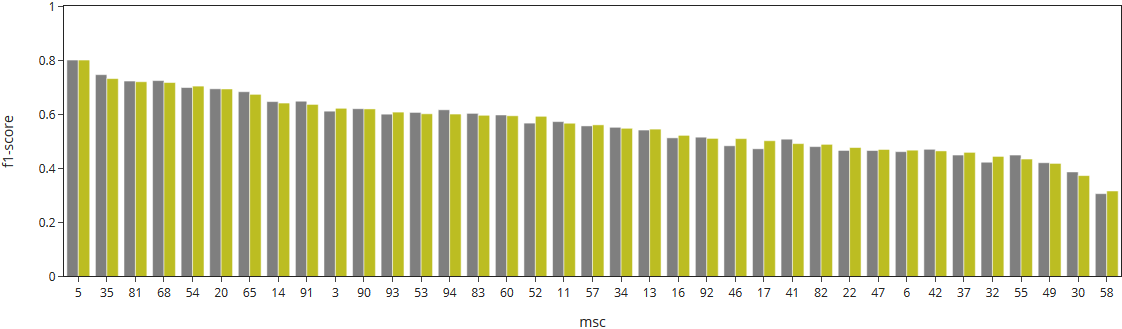
\includegraphics[width=\textwidth]{mathEncoding.png}
  \caption{Mathematical symbols in \texttt{title} and abstract \texttt{text} do not improve the classification quality. Method \texttt{uT1} =left bar; method \texttt{uM1}=right bar%TODO: change x axis label to pMSCn 
 }\label{fgMath}
  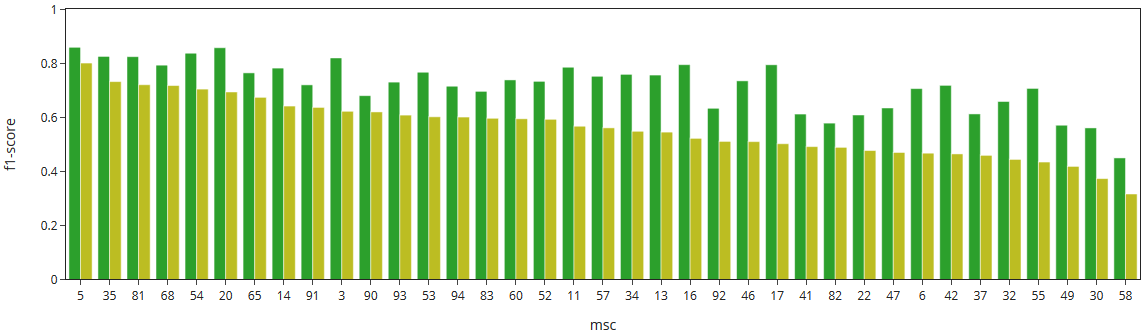
\includegraphics[width=\textwidth]{POSeffekt.png}
\caption{Part-of-speech tagging for mathematics does not improve the classification quality. Method \texttt{uM1}=left bar, method \texttt{tite}=right bar.}\label{fgPOS}
\end{figure}
By filtering out all mathematical expressions in the current production method \texttt{uT1} in contrast to \texttt{uM1} we have direct information about the impact of mathematical expressions on the classification quality.
We see that the overall $F_1$ score without mathematical expressions $f_\mathrm{uT1}=64.5\%$ is slightly higher than the score with mathematical expressions $f_\mathrm{uM1}=64.4\%.$ 
Here, the main effect is the increase of the recall from  $63.9\%$ to $64.2\%.$
Also a class-wise investigation shows that for most classes, the \texttt{uT1} outperforms \texttt{uM1}, cf., Figure \ref{fgMath}.
Exceptions are pMSCn 46 (Functional analysis ) and 17 (Nonassociative rings and algebras) where the inclusion of math tags raises the $F_1$-score slightly.

We evaluated the effect of the \emph{part of speech tagging} (POS), by comparing \texttt{tite} with \texttt{uM1}. $f_\mathrm{tite}=.713$ clearly outperforms $f_\mathrm{uM1}=.64.$ This is true for all MSC subjects, cf. Figure~\ref{fgPOS}. We modified posLingo to output the POS tagged text and used this text as input and retrained scikit learn classifier \texttt{tite2}. This did not improve the results over \texttt{tite}.

\paragraph{Effect of features and human baseline}
The newly developed method combined method~\cite{Scharpf2020} works best in a combined approach that uses \texttt{title}, abstract \texttt{text} and references \texttt{titer} $f_\mathrm{titer}=77.3\%.$
This method is significantly better than methods that omit a feature.
The best performing single feature method is \texttt{refs} $f_\mathrm{refs}=74.6\%$) followed by \texttt{text} $f_\mathrm{text}=69.9\%$ and \texttt{titls} $f_\mathrm{titls}=62.3\%$.
Thus generating the MSC subject from the references is an important strategy which can also be seen by comparing the score for the two combinations of features (\texttt{tiref} $f_\mathrm{text}=76\%$ and \texttt{teref} $f_\mathrm{text}=77\%$ vs \texttt{tite} $f_\mathrm{text}=71.3\%$).
However, the naive reference based method \texttt{ref1} $f_\mathrm{text}=65.2\%$ that is currently used in production, is worse than just using \texttt{tite} without references.
Thus training a machine learning algorithm that weights all information from the fine grained MSC codes is clearly better than the majority vote of the references, cf. \ref{fgRefs}.



\begin{figure}[t]
  \centering
  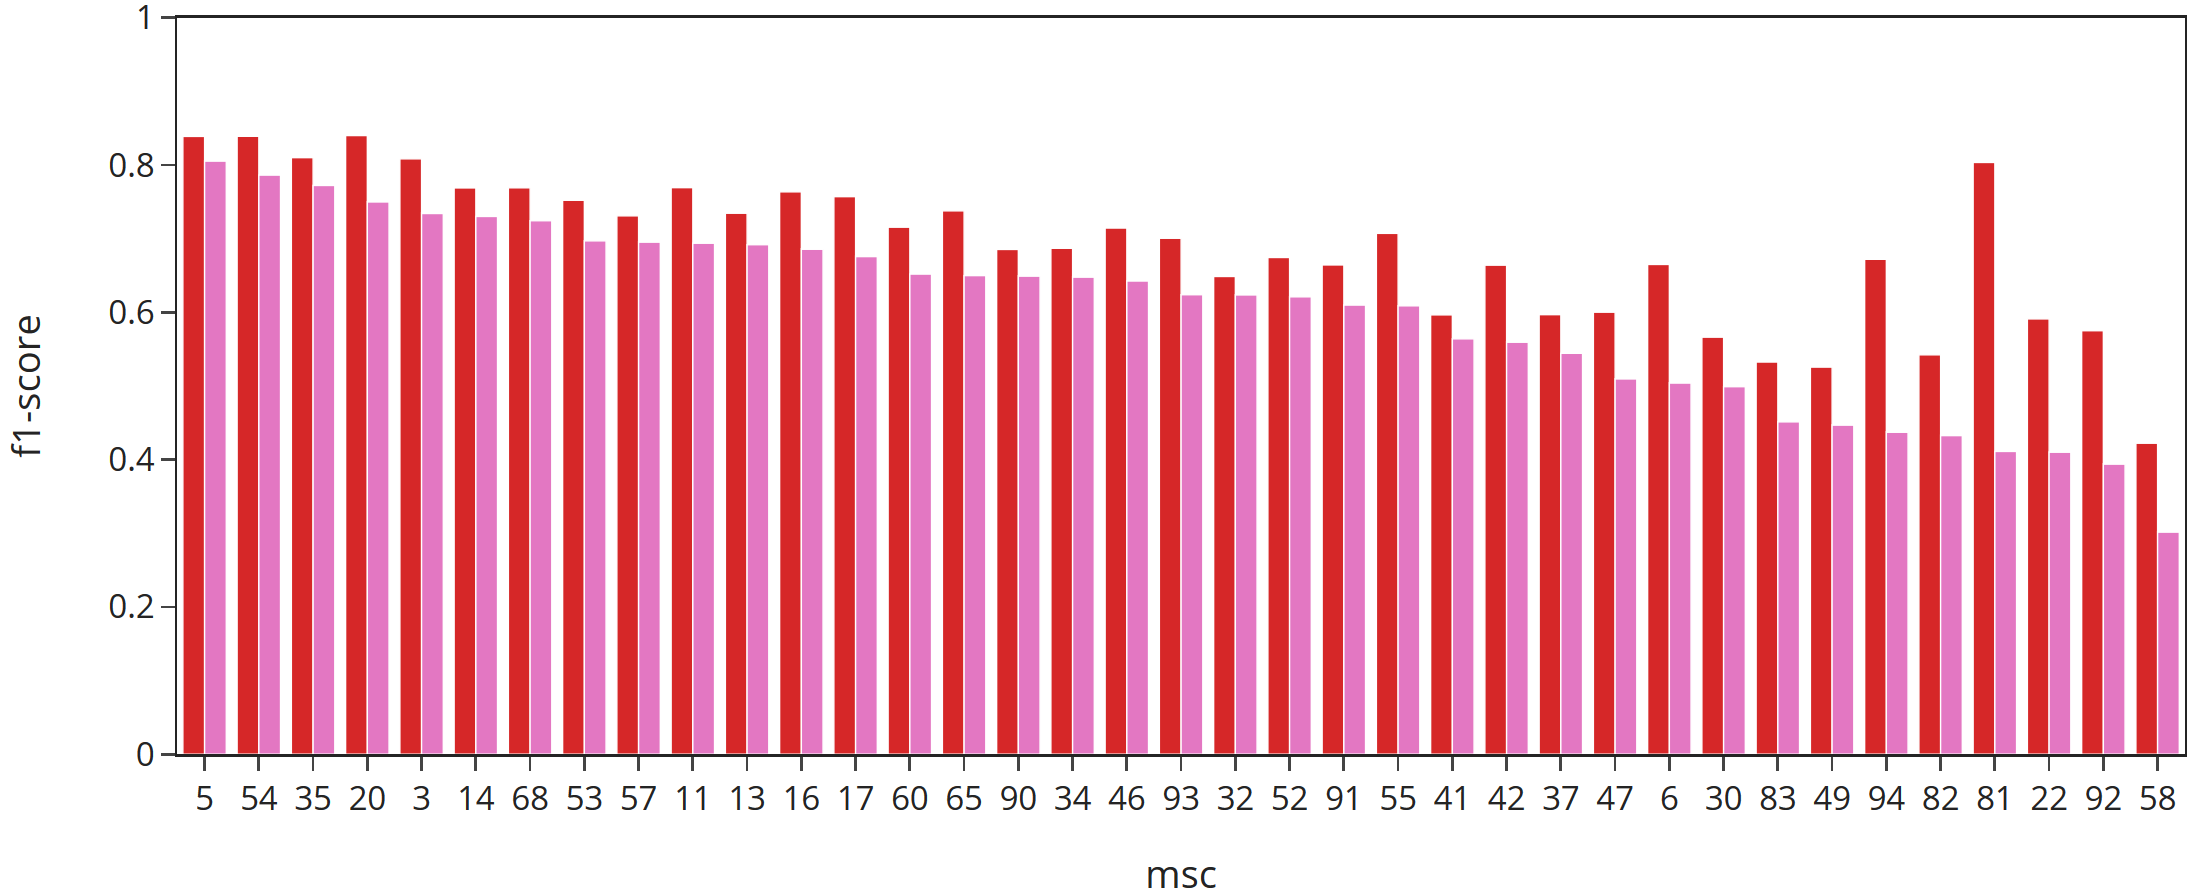
\includegraphics[width=1\textwidth]{ref1-refs.png}
  \caption{Machine learning method (\texttt{refs}, left)  clearly outperforms current production (\texttt{ref1}, right) method using references as only source for classification.}\label{fgRefs}
  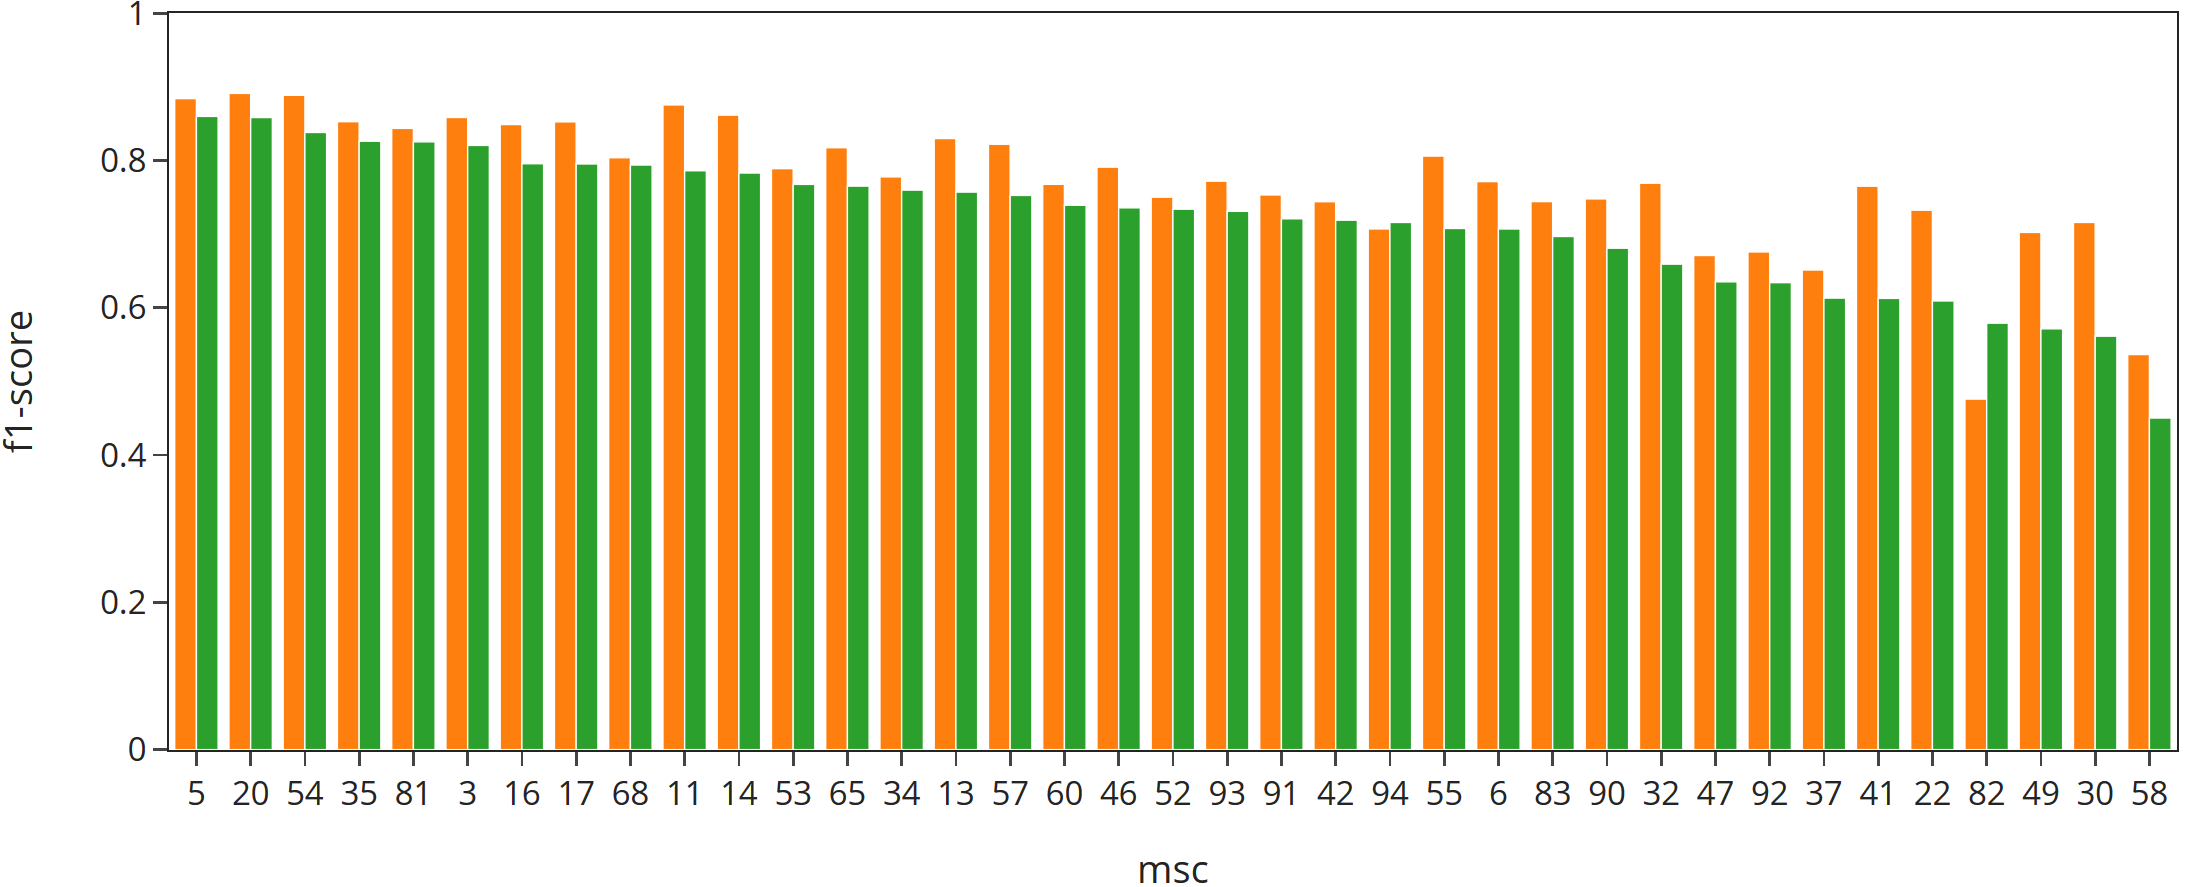
\includegraphics[width=1\textwidth]{mr1-titer.png}
  \caption{For many pMSCn the best automatic method (\texttt{titer}, right) gets close to the performance of the human baseline (\texttt{mr1} left)}\label{fgHum}
\end{figure}
Even the best performing machine learning algorithm, \texttt{titer} with $f_\mathrm{titer}=77.3\%$, is worth than using the classification by human experts from the other reviewing service MR \texttt{mr1} $f_\mathrm{mr1}=81.2\%.$ 
However, there is no basis to define which primary MSC subject, either from MR or zbMATH, is truly correct.
The assignment of a two digit label to a mathematical research paper that in most cases touches different aspects of mathematics, can not in all cases be classified into one of the classes.
While for some classes such as 20, the agreement is $89.1\%$ for other classes such as 82, it is only $47.6\%$ regarding the $F_1$ score, cf., Figure \ref{fgHum}.

We also investigated the bias introduced by the non random selection of the training set.
Performing ten fold cross validation on the entire dataset yields to a $f_\mathrm{titer,10}=.776$ with a standard deviation $\sigma_\mathrm{titer,10}=.002.$
Thus the selection of test set does not introduce a significant bias.

\begin{figure*}[t]
  \centering
  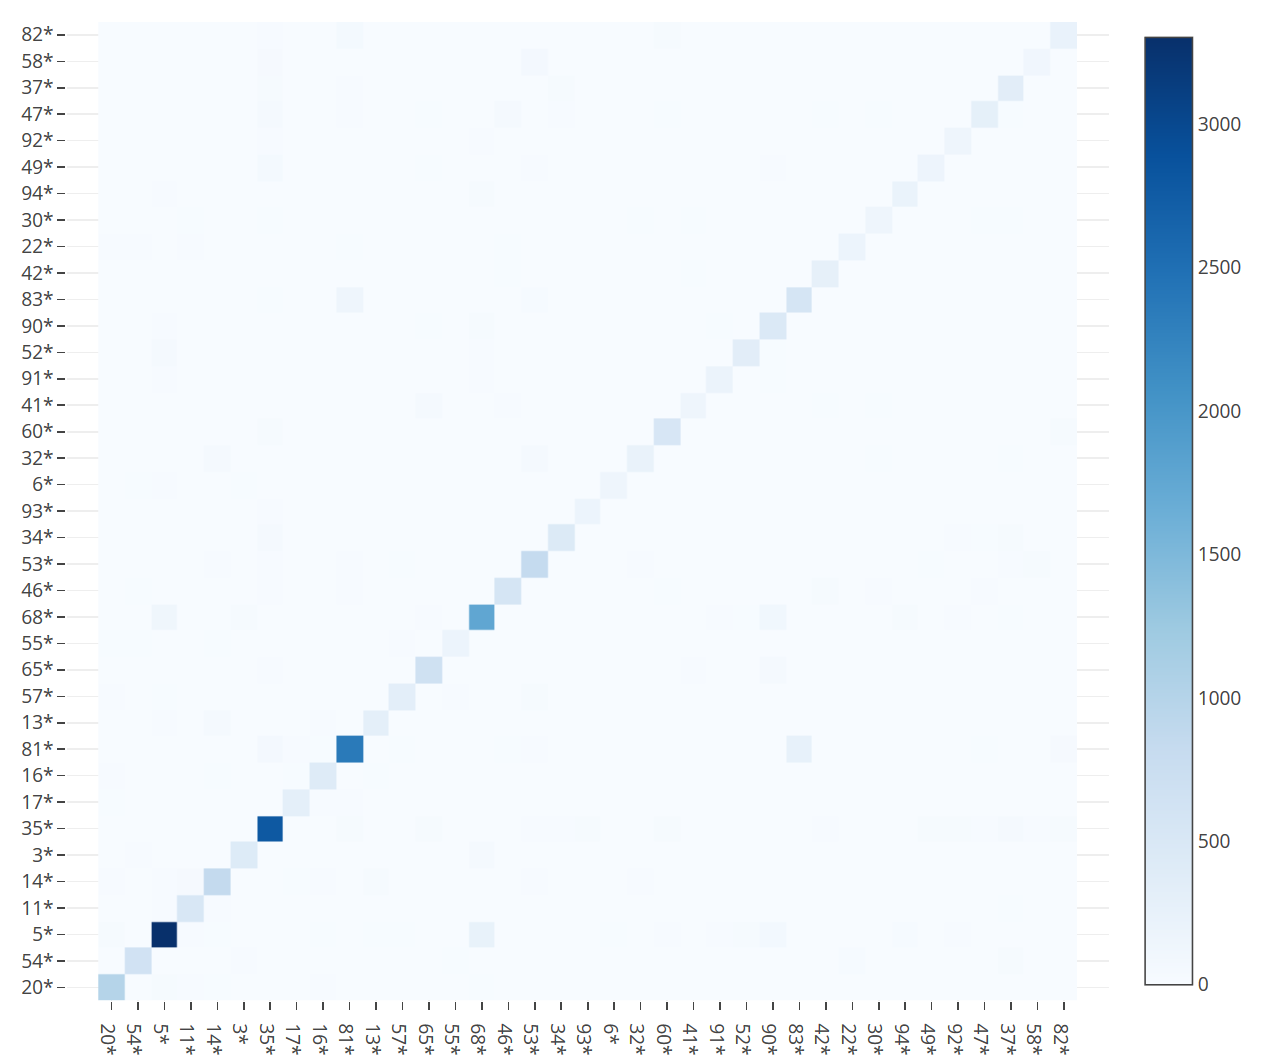
\includegraphics[width=.48\textwidth]{confusion.png}
  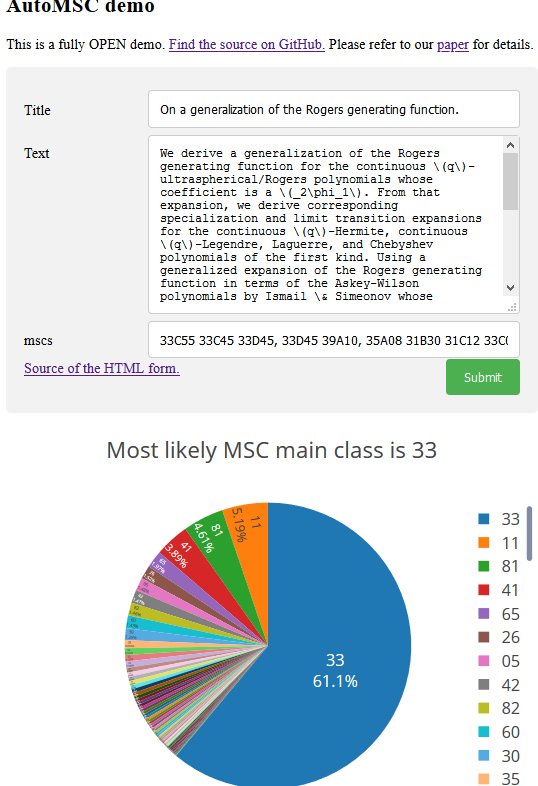
\includegraphics[width=0.48\textwidth]{webFrontend.png}
  \caption{Confusion matrix \texttt{titer} (left); classification frontend (right)}\label{fgScreenshot}\label{fgConfusion}
\end{figure*}
After having discussed the pros and cons of the various methods, we now discuss how the currently best performing method, \texttt{titer}, can be improved. 
One standard tool to analyze misclassifications is a confusion matrix, cf., Figure \ref{fgConfusion}.
In this matrix, off-diagonal elements of this matrix indicate that two classes are often mixed by the classification algorithm.
The x axis shows the true labels, whereas the y axis shows the predicted labels.
The most frequent error of \textit{titer} was that 68 (Computer science) was classified as 5 (Combinatorics).
Moreover, 81 (Quantum theory) and 83 (Relativity and gravitational theory) are mixed up often.


However, in general the number of misclassifications are small and there is no immediate action that one could do to avoid special cases of misclassification that do not involve a human expert.


Since \texttt{titer} outperforms both text-based and reference based methods currently used in zbMATH we decided to develop a restful API which wraps our trained model into a service.
We use pythons fastAPI under unicorn to handle higher loads.
%cite fastAPI and unicorn
Our system is available as a docker container and can thus be scaled on demand.
%maybe cite docker - although I think it could be like citing python
To simplify development and testing, we provide a static HTML page as micro UI.
This UI displays not only the most likely primary MSC subjects but also less likely MSC subjects.
We expect that this will support support human experts, if the most likely MSC subject seems inappropriate.
The result is displayed as a pie-chart, cf., Figure \ref{fgScreenshot} from
\url{https://automscbackend.formulasearchengine.com}.
To use the system in practice, an interface to the citation matching component of zbMATH would be desired to paste the actual references rather than the MSC subjects extracted from the references.
Moreover, looking at the precision recall curve (Figure \ref{fgPR}) for \texttt{titer}, suggests that one can also select a threshold for falling back to manual classification.
For instance, if one requires a precision that is as high as the precision of the other human classifications by MR, one would need to only consider suggestions with a score of $>0.5$. 
This would automatically classify $86.2\%$ of the annually 135k articles and thus significantly reduce the number of articles that a human needs to look at without a loss of classification quality.

\begin{figure}[t]
  \centering
  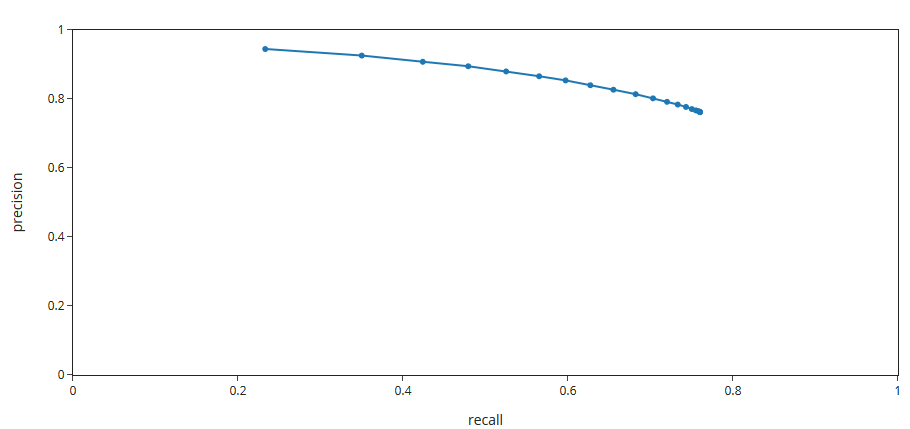
\includegraphics[width=.7\textwidth]{prcurve.png}
  \caption{Precision recall curve \texttt{titer}.}
  %very short caption and sparse plot
  \label{fgPR}
\end{figure}
This is something we might develop in the future.
% this refers to what?
% an issue we might tackle ...


\section{Conclusion \& Future Work}\label{sec.concl}
Returning to our research questions, we summarize our findings as follows:
\begin{enumerate}
  \item The quality of the classification for the primary MSC subject can be evaluated with classical information retrieval methods such as precision, recall and $F_1$-score.
%  The downside of binary evaluation approaches is that the degree of incorrectness is not taken into account.
%  % what do you mean by "incorrect"?
%  However, we could not agree on an automated non-strict evaluation measure. Overall, we see that the $F_1$ score matches the perceived quality of the results and we do not see a need to invent further evaluation methods at this point in time.
  \item In accordance with~\cite{Scharpf2020}, we did not find evidence that mathematical expressions improve pMSCn classification.
  \item We found that modern machine learning methods do not benefit from the POS tagging based model developed by \cite{SchonebergS14}.
  \item References have the highest prediction power, followed by abstract text and title.
  \item The best performing method has an $F_1$ score of 77.2\%.
  \item The manual classification is significantly better for most classes. However, the self reported score can be used to reduce the classification effort by 86.2\%, without a loss in classification quality.
\end{enumerate}

For the future, we plan to extend our work to full MSC codes.
Moreover, we would like to be able to assign pMSCn to document sections, since we realize that some research just does not fit into one of the classes.
Moreover, we will extend out field of application to other mathematical research artifacts such as blog posts, software, or dataset descriptions.
As next step, we plan to also generate pMSCn from authors using the same methods we applied for references.
We speculate that they will have a high impact on the classification as authors often publish in the same field.
Here, we are connecting with our research efforts on affiliation disambiguation that can be used as fallback for junior authors without a long track record.
Another extension is a better combination of the different features.
Especially for the full MSC code research we will need to use different encoding for the MSC from references and authors.
However, this new encoding requires more main memory for the model training and can not be done on a standard laptop.

\paragraph{Acknowledgments} This work was supported by the German Research Foundation (DFG grant GI 1259-1).
The authors would like to express their gratitude to Felix Hamborg, and Terry Ruas for their advice in the most recent machine learning technology.
\printbibliography[keyword=primary]
